\chapter{Parsers}
\label{chap:Parsers}
\theoremstyle{definition}
\begin{definition}[Parser]
    A parser is a program that : 
    \begin{itemize}
        \item Accepts/rejects input a sentence in the language (recognizer)
        \item Extracts a(n) (abstract) syntax tree
    \end{itemize}
\end{definition}
    \section{Parsing Tools}
        A parsing tool lets you create parsers. We can denote two kinds :
        Generator an Library. Note that is just a generalization. The main
        distinction to retain is the generation vs interpretation.

        Parsing tools are often called "parsers", it is acceptable, but
        incorrect, parsing tools create and/or run parsers.

        Parsing tools are compilers! 
        \begin{itemize}
            \item Language = grammar notation
            \item Code generation (parser generators) or interpretation (parsing
            libraries) (depending on the used tool)
            \item Domain Specific Language (DSL) (depending on how we define it.
            DSL is opposed to Turing-Complete language like Java, Ruby, Python,
            etc. A DSL could be XML, JSON, Grammar, SQL, etc.)
        \end{itemize}
        \subsection{Parsing Generator}
            Note : in the following figure, all solid boxes denote programs.
            \theoremstyle{definition}
            \begin{definition}[Parsing Generator]
                A Parsing Generator is :
                \begin{itemize}
                    \item Outputs a parser program (typically source code)
                    \item Typically a command line tool
                    \item Typically uses own grammar language
                \end{itemize}
            \end{definition}
            \begin{figure}[H]
                 \centering
                 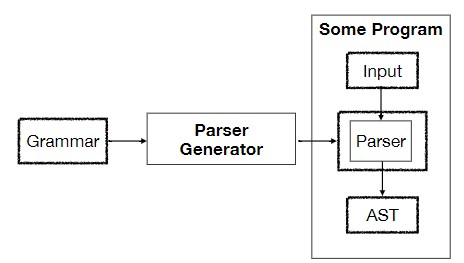
\includegraphics[scale=0.6]{Parser_Generator.jpg}
                 \caption{Parser Generator}
                 \label{fig:parser_gen}
            \end{figure}
        \subsection{Parsing Library}
            \theoremstyle{definition}
            \begin{definition}[Parsing Library]
                A Parsing Library is : 
                \begin{itemize}
                    \item Let us "interpret" a grammar
                    \item Grammar typically defined with a DSL.
                \end{itemize}
            \end{definition}
            \begin{figure}[H]
                 \centering
                 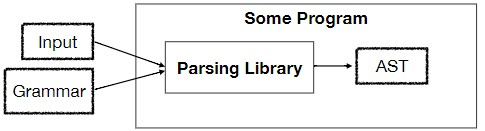
\includegraphics[scale=0.6]{Parser_Lib.jpg}
                 \caption{Parser Library}
                 \label{fig:parser_lib}
            \end{figure}
            Note that input AND grammar could be in the "Some Program" box.
    \section{(Abstract) Syntax Tree}
        \subsection{Syntax Tree}
            Remember the notation of figure \ref{fig:json_grammar} and
            \ref{fig:json_sentence}. To make it easier for Syntax Trees we will use
            the figure \ref{fig:bnf}. Doing so, we can extract the following ST : 
            \begin{figure}[H]
                \centering
                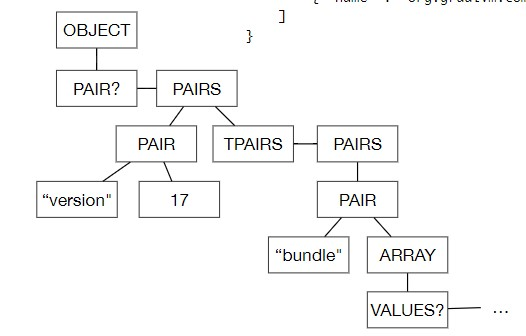
\includegraphics[scale=0.6]{SyntaxTree.jpg}
                \caption{Syntax Tree}
                \label{fig:syntax_tree}
            \end{figure}
            Syntax Tree is the following : for each phrase in the sentence we follow
            the grammar. It is the only thing we can do!
        \subsection{Abstract Syntax Tree}
            Here is the same Syntax Tree but abstracted : 
            \begin{figure}[H]
                 \centering
                 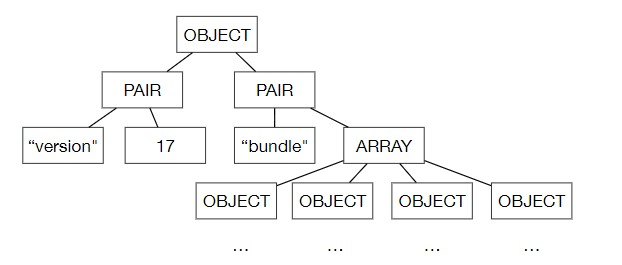
\includegraphics[scale=0.6]{AST_BIS.jpg}
                 \caption{Abstract Syntax Tree}
                 \label{fig:ast_bis}
            \end{figure}
            As we can see, it is much more clear than the classical Syntax Tree.

    \section{Summary 1}
    Parsing Tools that allow us to use grammar definition like PEG or EBNF (with
    more symbols that denotes more explicit stuffs) will generally produce
    better Syntax Tree than the others. However AST let us decide precisely what
    we want as node/leaves in the tree. Let's take an example using Java : 
    
    \begin{lstlisting}[language=Java]
        list.forEach(x -> System.out.println(x));
        list.reduce((x,y) -> x + y);
    \end{lstlisting}
    As we can see, the difference is that with 1 identifier we do not need
    parenthesis. That must be take into account when generating the Syntax Tree.
    It would lead to the following Syntax Trees : 
    \begin{figure}[H]
         \centering
         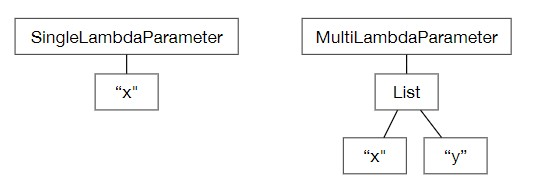
\includegraphics[scale=0.6]{ST_ex1.jpg}
         \caption{First ST}
         \label{fig:first_st}
    \end{figure}

    However, as we have seen, parsing is just the start of the pipeline! We have
    to do a lot of work with it (check for errors, generate bytecode, etc.).
    With this kind of Syntax Tree, we would have to deal with different kind of
    node for the same lambda principle. Using AST we can have the following : 
    \begin{figure}[H]
         \centering
         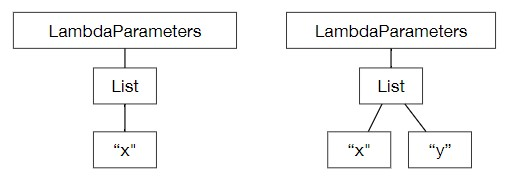
\includegraphics[scale=0.6]{ST_ex2.jpg}
         \caption{Second AST}
         \label{fig:second_ast}
    \end{figure}
    Which allow us to use the same code to deal with both!

    \section{Coding a parser}
        General principles : 
        \begin{itemize}
            \item One function per symbol (non-terminals \& terminals);
            \item Model in the input as globally accessible character array;
            \item The current input position is globally accessible;
            \item Calling a function = attempting to parse the symbol it denotes
            at the current input position;
            \item A parsing function returns : 
                \begin{itemize}
                    \item true if the symbol was matched, updating the input
                    position past the matched input.
                    \item false if they failed to match, the input remains
                    unchanged.
                \end{itemize}
        \end{itemize}
        See parser.java file. Note that, in order to be sure our implementation
        really work, we can use the debuger and check for the pos cursor at the
        end, or to go further we could also inspect the parse tree if we have
        build one. 

        As we can see, the parser we wrote is verbose and cumbersome. Also it
        does not have any bells or whistles, if it fails it just fails, it does
        not tell us where it fails or why. What we have done is implementing a
        PEG semantics for the grammar (hint, a* a is empty). Backtracking in PEG
        is to reset the counter before the start of the sequence. CFG also have
        a backtracking technique but it is not the same.

        We can also add AST to our parser. In order to do that in Java, we just
        need to add a Dequeue and modify only a few methods. See parser\_ast.java
        for that.

    \section{Parser Combinator}
        The parser we have implemented from PEG grammar. As we have seen, this
        parsers have a lot of duplication (each "expression" is handled the same
        way). The idea to solve that is to build an AST where each node is an
        "expression" and interpret it.

        The idea, is that each combinator is a node/parsing expression in the
        AST. See file Combinators.java. Using combinators allow us to cut down
        on verbosity \& code duplication (across all grammars and within a
        specific grammar). However it still have some drawbacks : 
        \begin{itemize}
            \item Harder to debug
            \item It's slower because of megamorphism (we'll come back later on
            this)
        \end{itemize}
        Note that theses issues can be eliminated by using combinators for code
        generation. Good frameworks (like Autumn) will mitigate usability
        issues.